\newpage
\section{Vorbereitungsfragen}
\subsection{1}
\begin{figure}[H]
    \centering
    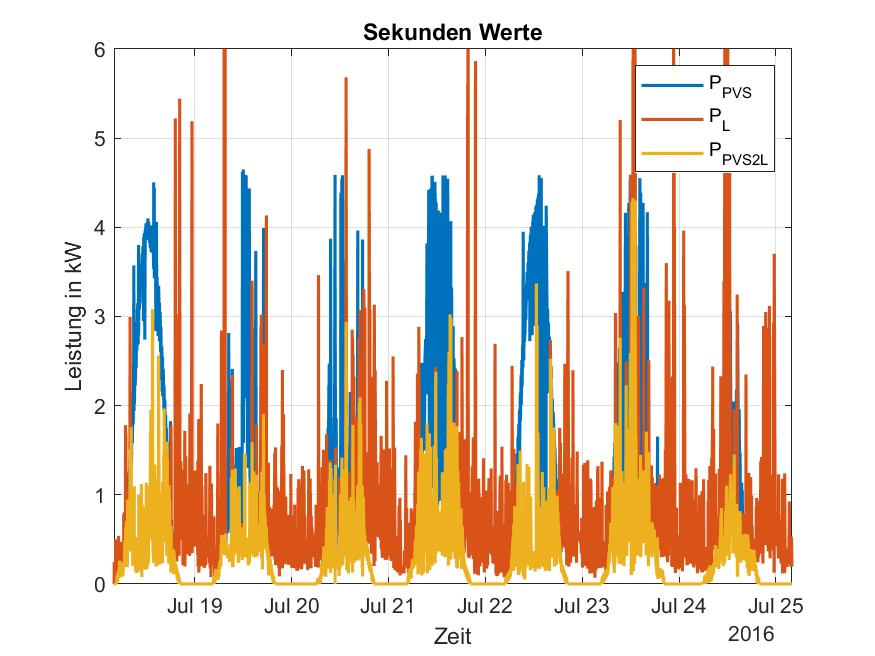
\includegraphics[width=\textwidth]{Abbildungen/plot.jpg}
    \caption{Beschreibung des Plots}
    \label{fig:plot3062023}
\end{figure}
\subsection{2}
$E.E_pvs = sum(ts.Ppvs/1000)/3600=149,96kWh;\\
E.E_l = sum(ts.Pl/1000)/3600=89,08kWh;\\
E.E_pvs2l = sum(Ppvs2l/1000)/3600=41,52kWh;$\\

\subsection{3}
\begin{figure}[H]
    \centering
    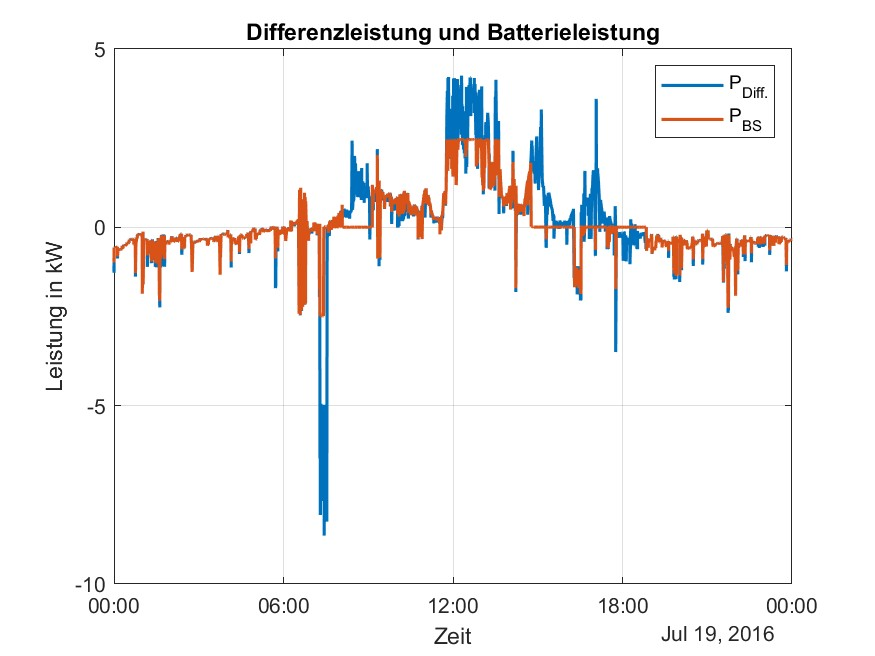
\includegraphics[width=\textwidth]{Abbildungen/plot_vorbereitungsfrage3.jpg}
    \caption{Beschreibung des Plots}
    \label{fig:plot3062023}
\end{figure}
\subsection4}
\begin{figure}[H]
    \centering
    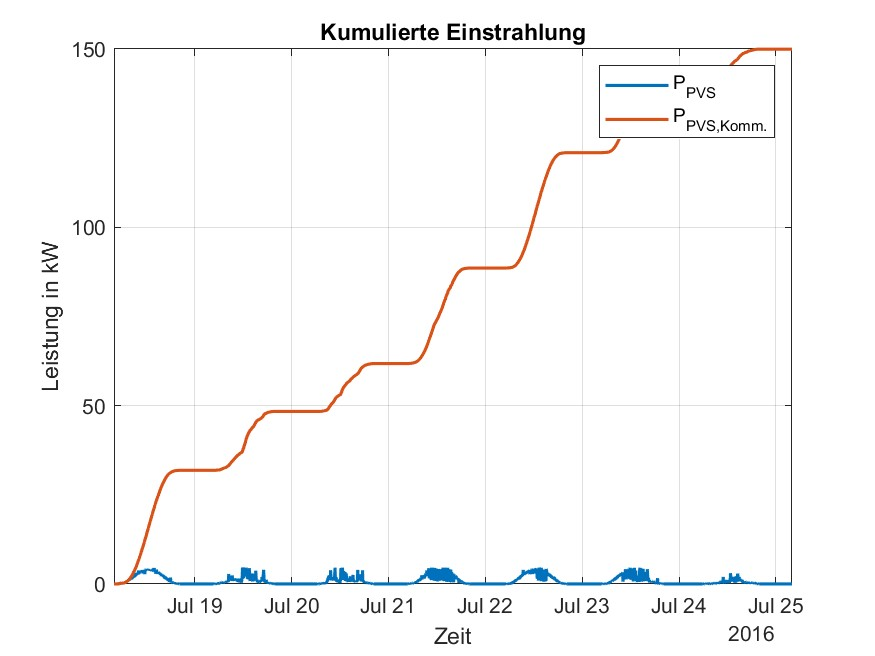
\includegraphics[width=\textwidth]{Abbildungen/plot_vorbereitungsfrage4.jpg}
    \caption{Beschreibung des Plots}
    \label{fig:plot3062023}
\end{figure}